%%%%%%%%%%%%%%%%%%%%%%%%%%%%%%  IEEEsample2e.tex %%%%%%%%%%%%%%%%%%%%%%%%%%%%%%
%% changes for IEEEtrans.cls marked with !PN
%% except all occ. of IEEEtran.sty changed IEEEtran.cls
%%%%%%%%%%                                                       %%%%%%%%%%%%%
%%%%%%%%%%    More information: see the header of IEEEtran.cls   %%%%%%%%%%%%%
%%%%%%%%%%                                                       %%%%%%%%%%%%%
%%%%%%%%%%%%%%%%%%%%%%%%%%%%%%%%%%%%%%%%%%%%%%%%%%%%%%%%%%%%%%%%%%%%%%%%%%%%%%%


\documentclass[conference]{template/IEEEtran} %!PN
%\documentclass[12pt,draft]{IEEEtran} %!PN
%\documentstyle[twocolumn]{IEEEtran}
%\documentstyle[12pt,twoside,draft]{IEEEtran}
%\documentstyle[9pt,twocolumn,technote,twoside]{IEEEtran}
\usepackage[T1]{fontenc}
\usepackage[scaled]{beramono} % important for nicer code font
\usepackage{listings} 
\usepackage{pbox}
\usepackage{tikz}
\usepackage{etoolbox}
\usepackage{amsmath}
\usepackage{amssymb}
\usepackage[nolist,printonlyused]{acronym}
\usepackage{hyperref}
\usepackage{listings} 
\usepackage{etoolbox}
\usepackage{tikz}
\usepackage{soul}  
\usepackage{color}

\definecolor{amber}{rgb}{1.0, 0.75, 0.0}
\definecolor{applegreen}{rgb}{0.55, 0.71, 0.0}
\definecolor{burntsienna}{rgb}{0.91, 0.45, 0.32}
\definecolor{cyan}{rgb}{0.0, 1.0, 1.0}
\definecolor{brandeisblue}{rgb}{0.0, 0.44, 1.0}

\lstset{
basicstyle=\ttfamily\color{black}, 
keywordstyle=\color{black}\bfseries,       
% keywordstyle=\color{javadocblue},     
commentstyle=\color{black},              
numbers=none,                           
numberstyle=\tiny,                      % Line-numbers fonts
stepnumber=1,                           % Step between two line-numbers
numbersep=5pt,                          % How far are line-numbers from code
backgroundcolor=\color{white}, % Choose background color
tabsize=2,     
frame=none,
%xleftmargin=1.5mm,
%xrightmargin=1.5mm,
captionpos=b,   
keepspaces=true,
xleftmargin=1.5mm,
xrightmargin=1.5mm,                        % Caption-position = bottom
breaklines=true,                        % Automatic line breaking?
breakatwhitespace=false,                % Automatic breaks only at whitespace?
showspaces=false,                       % Dont make spaces visible
showtabs=false,                         % Dont make tabls visible
columns=flexible,                       % Column format
morekeywords={}  
} 
 
 \lstdefinelanguage{debuggerTesting}
{keywords={},
% otherkeywords={::,:,->,=>,[,],;,==;+=,=,:<=:,:==:,<,+,&,!,\,,*},
otherkeywords={[,]},
alsodigit={0,1,2,3,4,5,6,7,8,9,0},
stringstyle=\color{green},
mathescape=true,
showstringspaces=false,
sensitive=true,
tabsize=2,
columns=fullflexible,
morestring=[b]",
comment=[l]{//},
basicstyle=\scriptsize\ttfamily\color{darkgray},
keywordstyle=\bf\scriptsize\ttfamily\color{black},
}


\lstdefinelanguage{reducedMbeddr}
{keywords={},
% otherkeywords={::,:,->,=>,[,],;,==;+=,=,:<=:,:==:,<,+,&,!,\,,*},
otherkeywords={},
alsodigit={0,1,2,3,4,5,6,7,8,9,0},
stringstyle=\color{green},
mathescape=true,
showstringspaces=false,
sensitive=true,
tabsize=2,
columns=fullflexible,
morestring=[b]",
comment=[l]{//},
basicstyle=\scriptsize\ttfamily\color{darkgray},
keywordstyle=\bf\scriptsize\ttfamily\color{black},
}

\lstdefinelanguage{mbeddr}
{keywords={return,test,case,exported,int8_t,foreach,it,int32,void,sized,assert,rule,as,
applicable,concept,overrides,do,typeof,if,applicable,error,int64_t,int8, for,
concepts,constraints,can,be,child,ancestor,isNotNull,node,int32_t,executeTests,
for,string,foreach
% assert(0),assert(1),assert(2),assert(3),assert(4),
% assert(5),assert(6),assert(7),assert(8),assert(9),assert(10),assert(11),assert(12),
% assert(13),assert(14),assert(15),assert(16),assert(17),assert(18),assert(19),assert(20),
% assert(21),assert(22),assert(23),assert(24),assert(25),assert(26),assert(27),assert(28),
% assert(29),assert(30)
},
% otherkeywords={::,:,->,=>,[,],;,==;+=,=,:<=:,:==:,<,+,&,!,\,,*},
otherkeywords={},
alsodigit={0,1,2,3,4,5,6,7,8,9,0},
stringstyle=\color{black},
mathescape=true,
showstringspaces=false,
sensitive=true,
tabsize=2,
columns=fullflexible,
morestring=[b]",
comment=[l]{//},
basicstyle=\scriptsize\ttfamily\color{darkgray},
keywordstyle=\bf\scriptsize\ttfamily\color{black},
}
\lstdefinelanguage{constraintsAndTS}
{keywords={typeof,check,concept,ancestor,isNotNull,parentNode
% assert(0),assert(1),assert(2),assert(3),assert(4),
% assert(5),assert(6),assert(7),assert(8),assert(9),assert(10),assert(11),assert(12),
% assert(13),assert(14),assert(15),assert(16),assert(17),assert(18),assert(19),assert(20),
% assert(21),assert(22),assert(23),assert(24),assert(25),assert(26),assert(27),assert(28),
% assert(29),assert(30)
},
% otherkeywords={::,:,->,=>,[,],;,==;+=,=,:<=:,:==:,<,+,&,!,\,,*},
otherkeywords={;,:,=,<,>,+},
alsodigit={0,1,2,3,4,5,6,7,8,9,0},
stringstyle=\color{black},
mathescape=true,
showstringspaces=false,
sensitive=true,
tabsize=2,
columns=fullflexible,
morestring=[b]",
comment=[l]{//},
basicstyle=\scriptsize\ttfamily\color{darkgray},
keywordstyle=\bf\scriptsize\ttfamily\color{black},
}

\lstdefinelanguage{debuggerDSL}
{keywords={contribute,frame,mapping,name,break,on,nodes,to,step-into,node,hide,
with,identifier,for
% assert(0),assert(1),assert(2),assert(3),assert(4),
% assert(5),assert(6),assert(7),assert(8),assert(9),assert(10),assert(11),assert(12),
% assert(13),assert(14),assert(15),assert(16),assert(17),assert(18),assert(19),assert(20),
% assert(21),assert(22),assert(23),assert(24),assert(25),assert(26),assert(27),assert(28),
% assert(29),assert(30)
},
% otherkeywords={::,:,->,=>,[,],;,==;+=,=,:<=:,:==:,<,+,&,!,\,,*},
otherkeywords={;,:},
alsodigit={0,1,2,3,4,5,6,7,8,9,0},
stringstyle=\color{black},
mathescape=true,
showstringspaces=false,
sensitive=true,
tabsize=2,
columns=fullflexible,
morestring=[b]",
comment=[l]{//},
basicstyle=\scriptsize\ttfamily\color{darkgray},
keywordstyle=\bf\scriptsize\ttfamily\color{black},
}

\newcommand{\lcolorbox}[2]{%
  \hspace*{-\fboxsep}\colorbox{#1}{#2}%
}

\definecolor{grayx11gray}{rgb}{0.75, 0.75, 0.75}
\definecolor{lavendergray}{rgb}{0.77, 0.76, 0.82}
\definecolor{lightslategray}{rgb}{0.47, 0.53, 0.6}
\definecolor{pastelgray}{rgb}{0.81, 0.81, 0.77}

\definecolor{g1}{HTML}{8C8C8C}
\definecolor{g2}{HTML}{969696}
\definecolor{g3}{HTML}{ABABAB}
\definecolor{g4}{HTML}{B8B8B8}
\definecolor{g5}{HTML}{C9C9C9}
\definecolor{g6}{HTML}{D6D6D6}
\definecolor{g7}{HTML}{E5E5E5}
\definecolor{g8}{HTML}{F5F5F5}

\newcommand{\changefont}[3]{\fontfamily{#1}\fontseries{#2}\fontshape{#3}\selectfont}
\newcommand\change{}
%\newcommand{\mynote}[2]{}
\newcommand{\mynote}[2]{\textbf{{#1}(}\textit{{#2}}\textbf{)}}
\newcommand\todo[1]{\mynote{TODO}{#1}} 
\newcommand\kolja[1]{\mynote{KOLJA}{#1}} 
\newcommand\parhead[1]{\vspace{0.1cm}\noindent\textbf{{#1}}\ \ }  
\newcommand{\eg}{e.\,g., }
\newcommand{\ie}{i.\,e., }
\newcommand{\ic}[1]{\changefont{cmtt}{m}{n}{#1}\normalfont}
\newcommand{\lcr}[1]{\changefont{cmtt}{m}{n}{#1}\normalfont}
\newcommand{\sect}[1]{Section~\ref{#1}}
\newcommand{\fig}[1]{Fig.~\ref{#1}}
\newcommand{\lst}[1]{Listing~\ref{#1}}

\begin{document}

%\title{Using the Style File IEEEtran.sty} 
\title{Testing Debuggers for Extensible Languages} %!PN

\author{\IEEEauthorblockN{Domenik Pavletic}
\IEEEauthorblockA{itemis AG\\
Stuttgart, Germany\\
pavletic@itemis.com
}
\and
\IEEEauthorblockN{Kolja Dummann}
\IEEEauthorblockA{itemis AG\\
Stuttgart, Germany\\
dummann@itemis.com
}
\and
\IEEEauthorblockN{Syed Aoun Raza}
\IEEEauthorblockA{Stuttgart, Germany\\
aoun.raza@gmail.com}
}

\maketitle

\begin{abstract}
bla
\end{abstract}

\begin{IEEEkeywords}
% those terms are not on the IEEE keyword index:
%Extensible Languages, Domain-Specific Languages, Debuggers, Testing.
Formal languages, Software debugging, Software testing.
\end{IEEEkeywords}


% resulting table
\begin{acronym}[IDEIDEIDEIDEIDSSD]
 \setlength{\itemsep}{-0.2cm}
 \acro{SDF}{Syntax Definition Formalism}
 \acro{LLVM}{Low Level Virtual Machine}
 \acro{LLDB}{Low Level Debugger} 
 \acro{ASF}{Algebraic Specification Formalism}
 \acro{IDE}{Integrated Development Environment}
 \acro{KRoC}{Kent Retargetable occam Compiler}
 \acro{CSP}{Communicating Sequential Processes}
 \acro{Tcl}{Tool command language}
 \acro{AST}{Abstract Syntax Tree} 
 \acro{LWES}{Language Workbenches for Embedded Systems}
 \acro{DSL}{Domain-Specific Language}
 \acro{MPS}{Meta Programming System} 
 \acro{CDT}{C/C++ Development Tooling}
 \acro{GDB}{GNU Debugger}
 \acro{JPDA}{Platform Debugger Architecture}
 \acro{JDWP}{Java Debugging Wire Protocol}
 \acro{JDB}{Java Debugger}
 \acro{CPU}{Central Processing Unit} 
 \acro{EPL}{Eclipse Public License}
 \acro{MI}{Machine Interface}
 \acro{LOP}{Language Oriented Programming}
 \acro{RUP}{Rational Unified Process}
 \acro{xUML}{Executable UML}
 \acro{UML}{Unified Modeling Language}
 \acro{SQL}{Structured Query Language}
 \acro{GPL}{General Purpose Language}
 \acro{OS}{Operating System}
 \acro{API}{Application Programming Interface}
 \acro{GUI}{Graphical User Interface}
 \acro{ASCET}{Advanced Simulation and Control Engineering Tool}
 \acro{MDA}{Model-Driven Architecture}
 \acro{MDSD}{Model-Driven Software Development}
 \acro{JTAG}{Joint Test Action Group}
 \acro{XML}{Extensible Markup Language}
 \acro{VM}{Virtual Machine}
 \acro{JVM}{Java Virtual Machine} 
 \acro{UI}{User Interface}
 \acro{DWARF}{Debugging With Attributed Record Formats}
 \acro{LWC}{Language Workbench Challenge}
\end{acronym}
\section{Introduction}

Software development faces the challenge that \acp{GPL}
do not provide the appropriate abstractions for domain-specific problems. 
Traditionally there are two  
approaches to overcome this issue. One is to use frameworks 
that provide domain-specific abstractions expressed with a \ac{GPL}.
This approach has very limited support for static semantics, \eg 
no support for modifying constraints or type system.
% first appraoch is about internal DSLs?
The second approach is to use external \acp{DSL} for 
expressing solutions to domain problems. This approach 
has some other drawbacks: 
these \acp{DSL} are not inherently extensible.
% what was here: monolithic, all in advanced, central, foo bar
Extensible languages solve these problems. Instead of having a single 
monolithic \ac{DSL}, extensible languages enable modular and 
incremental extensions of a host language with domain specific 
abstractions~\cite{Voelter2011}.

To make debugging extensible languages useful to the language user, it is not
enough to debug programs after extensions have been translated back to the host 
language (using an existing debugger for the base language).  
A debugger for an extensible language must be extensible as well, to support
debugging of modular language extensions at the same abstraction level
(extension-level).
Minimally, this means users can step through constructs 
provided by the extension and see watch expressions (\eg variables) related to
the extensions.

% fix this part (we might have a fitting sentence somewhere)
Because language extensions can be based on other extensions and languages
evolve over time, it is essential to constantly test if debugger
behavior matches the expected behavior. To test debugging
behavior, a \ac{GPL} can be used, however this raises
the same issues discussed above. 
% ToDo: double check it!
We therefore propose in this paper \emph{DeTeL} (Debugger Testing Language), an
extensible \ac{DSL} for testing debuggers. 

\section{mbeddr}


The mbeddr open-source project\footnote{ \url{http://mbeddr.com}} 
focuses on supporting embedded software
development. It introduces a set of of modular domain-specific extensions
to C and also supports other languages for addressing common problems 
in software development, \eg writing documentation with close 
integration to code or capturing requirements. mbeddr is build using 
JetBrains \ac{MPS} language 
workbench\footnote{ \url{https://www.jetbrains.com/mps/}}.
\fig{mbeddrArch} shows how mbeddr is organized into layers, with \ac{MPS} at
the bottom and custom language extensions on top.
\ac{MPS} supports the definition, 
composition and use of general purpose or domain-specific languages. 
To archive this \ac{MPS} uses a projectional editor, this means, even 
if the notation might look textual it is not represented as a sequence 
of characters, which are transformed into a \ac{AST} by parsing. 
In contrast user actions manipulate the \ac{AST} directly. The \ac{AST} 
is then rendered to the user according to editor specifications/projection
rules. These rules are not limited to textual notations, for example can tabular
or mathematical notations can be used if appropriated. Since no parsing ambiguities 
can occur a wide range of languages extension can be supported.

\begin{figure}[h]
  \vspace{-2mm}
  \centering
    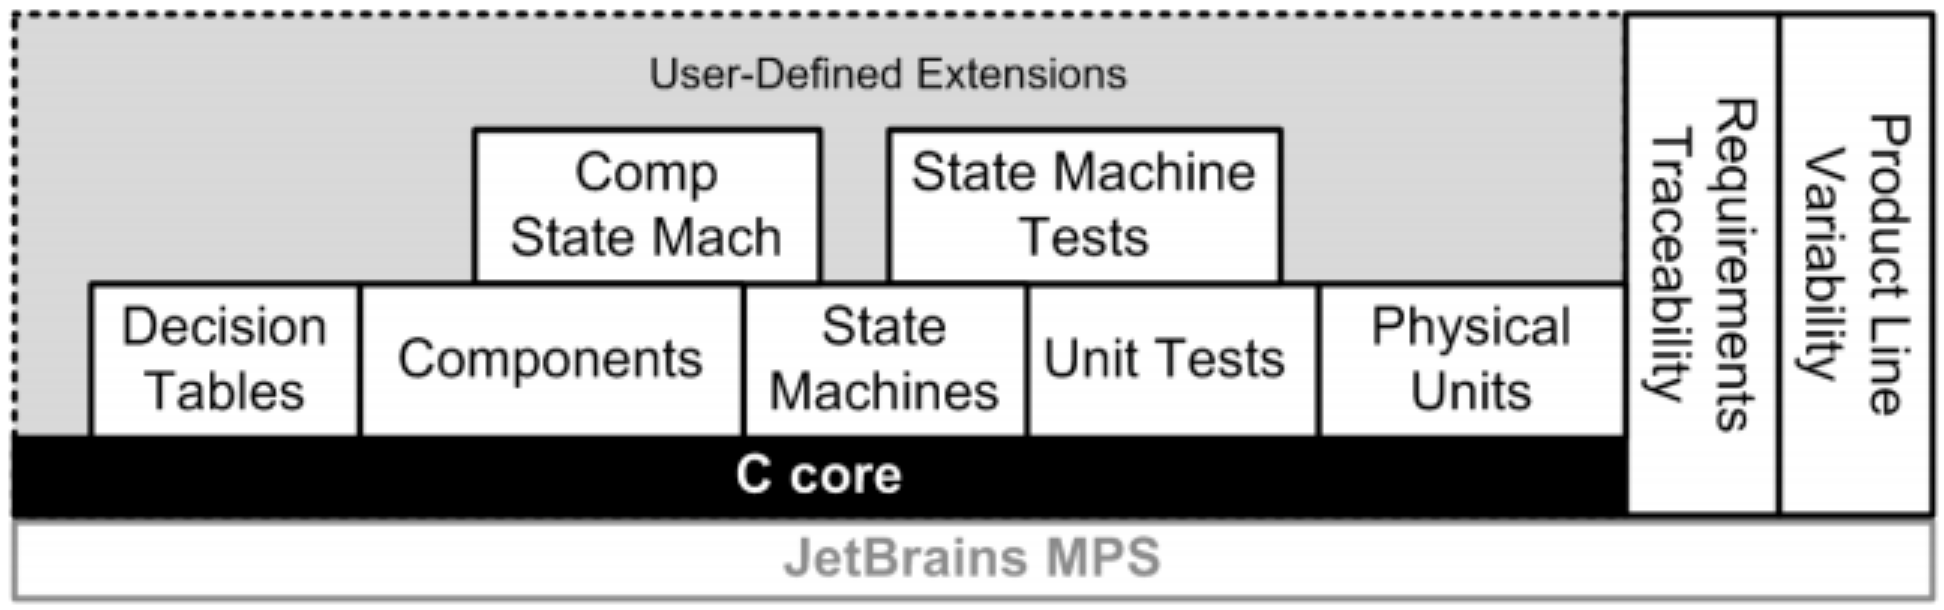
\includegraphics[width=8.5cm]{./figures/mbeddArch.png} 
    \vspace{-2mm}
    \caption{mbeddr language architecture~\cite{Voelter:2012:MEC:2384716.2384767}}
  \label{mbeddrArch}
  \vspace{-2mm}
\end{figure}


\subsection{Languages}
\label{languageImplementation}
mbeddr includes a extensible C99 implementation. In addition to plain C 
mbeddr also include a set of predefined extension on top of C. These 
extension include test cases, state machines, components and physical units. 
In \ac{MPS} languages are separated into modular aspects. The major aspects 
of a language are:  

\parhead{Structure:} Definition of the \ac{AST} of the language.

\parhead{Editor:} Projection rules how the \ac{AST} is presented to the user and how the user interacts with the program.

\parhead{Type System/Contraints:} Static semantics of the language.
 
\parhead{Generator:} Dynamic semantics of the language, transforms the model into executable code.

\subsection{Unit Test Language Extension}

This section shows the implementation of a minimal unit test language for
writing test cases with mbeddr. \lst{lst:generatedUT} shows a code
snippet.

\noindent 
\begin{minipage}[t]{120pt} 
\begin{lstlisting}[language=reducedMbeddr]
int32 main(int32 argc,
		string[] argv) {
   return $\colorbox{g1}{test[}$$\colorbox{g6}{forTest}$$\colorbox{g1}{]}$;
}
$\colorbox{white}{\hspace{2mm}{\color{white}\_fails;}}$
$\colorbox{white}{\hspace{2mm}{\color{white}blockexpr\_2();}}$
$\colorbox{white}{\hspace{2mm}{\color{white}\}}}$
$\colorbox{white}{\hspace{2mm}{\color{white}\}}}$
$\colorbox{white}{\hspace{2mm}{\color{white}int32\_t bp\_2() \{}}$ 
$\colorbox{white}{\hspace{2mm}{\color{white}i32\_t \_fails = 0;}}$		



$\colorbox{g7}{testcase forTest \{}$ 
$\colorbox{white}{\hspace{2mm}{\color{white}|}}$
   int32 sum = 0;
   int32[] nums = {1, 2, 3};
   for(int32_t i=0;i<3;i++){
     sum += nums[i];
   }
$\colorbox{g3}{\hspace{2.5mm}assert-equals sum == 3;}$
$\colorbox{white}{{\color{white}\_fails++;}}$
$\colorbox{white}{\hspace{5mm}{\color{white}pf("fal:\%d!3");}}$
$\colorbox{white}{\hspace{2mm}{\color{white}\}}}$
$\colorbox{white}{\hspace{2mm}{\color{white}return \_fails;}}$
$\colorbox{g7}{\}}$
\end{lstlisting}
\end{minipage} 
\hfill 
\rule[-61ex]{0.2ex}{27.2em}
\begin{minipage}[t]{130pt} 
\begin{lstlisting}[language=reducedMbeddr]
int32_t main(int32_t argc,
		char *(argv[])) {
   return $\colorbox{g1}{blockexpr\_2()}$;
}  
$\colorbox{white}{\hspace{2.5mm}{\color{white}|}}$
$\colorbox{g1}{int32\_t blockexpr\_2(void) \{}$
$\colorbox{g1}{\hspace{2.5mm}int32\_t \_fails = 0;}$
$\colorbox{g6}{\hspace{2.5mm}\_fails += test\_forTest();}$
$\colorbox{g1}{\hspace{2.5mm}return \_fails;}$
$\colorbox{g1}{\}}$



$\colorbox{g7}{int32\_t test\_forTest() \{}$
$\colorbox{g7}{\hspace{2.8mm}int32\_t \_fails = 0;}$
   int32_t sum = 0;
   int32_t[] nums = {1, 2, 3};
   for(int32_t i=0;i<3;i++){
     sum += nums[i];
   }
$\colorbox{g3}{\hspace{2.8mm}if (!(sum == 3)) \{}$
$\colorbox{g3}{\hspace{5.8mm}\_fails++;}$
$\colorbox{g3}{\hspace{5.8mm}printf("fail:\%d!=3",sum);}$
$\colorbox{g3}{\hspace{2.8mm}\}}$
$\colorbox{g7}{\hspace{2.8mm}return \_fails;}$
$\colorbox{g7}{\}}$
\end{lstlisting}
\end{minipage} 
\vspace{-1mm}
\begin{lstlisting}[caption=Example mbeddr program using the unit test language
on the left and the C code that has been generated from it on the right.,
language=mbeddr,label=lst:generatedUT]
\end{lstlisting}


\section{mbeddr Debugger}

\subsection{Architecture}
how does the debugger work


\subsection{Building Debugging Behavior}
show how debug support is build for foreach and unit test language

\section{Requirements on the Testing Language}

Our testing \ac{DSL} targets debuggers for imperative extensible languages.
Those debuggers usually provide at least the following functionality:
show the call stack and program state in relation to the languages used, 
suspend the debugger on breakpoints and offer the possibility to 
step through the code. Our testing language should allow us to test exactly those
four aspects. We have therefore defined the following functional and
non-functional requirements on the \ac{DSL}, which we will later implement in
our language. While some of those requirements are optional, we consider most of
them as mandatory.

\subsection{Functional Requirements}

The following list discusses the functional requirements we expect from a
testing language for debuggers. While \hyperref[FR3]{FR3} is considered
optional and \hyperref[FR3]{FR3} is mandatory in the embeded software domain, we
expect \hyperref[FR1]{FR1} and \hyperref[FR2]{FR2} to be essential.
 
\noindent \textbf{\label{FR1}FR1 Debug state validation:} In our test cases we
must be able to validate the call stack, and for each of its frames 
the program state and the location where suspended. 

The stack itself should be validated by specifying the expected stack frames and
their respective names. In terms of program state, we need to verify the names 
of watchables and their respective values, with can either be simple or complex.
Finally, location where suspended is a reference to a location inside the program under tests. 

\noindent \textbf{\label{FR2}FR2 Debugger control:} In order to test stepping
commands and breakpoints, we need the ability to specify stepping commands
(in, over and out) and locations where to break.

In a debugger test cases,
first, the location where to break is specified. Next, after suspending on this
location, an otional list of stepping commands is executed. Finally, after
suspending, specified validation rules are evaluated.

\noindent \textbf{\label{FR2}FR2 Automated test execution:} Since we can write
many different debugger tests, we require the ability to integrate our 
tests into an automatic execution environemt. This environment can be, \eg
an \ac{IDE} or a command-line tool. Latter is prefered, since it can be
executed on the local machine or on a build server.

\noindent \textbf{\label{FR3}FR3 Exchangeability of debugger backends:}
mbeddr targets the embedded domain and C. In this domain, target platforms and
vendors require different compilers and debuggers. 
Hence, we require the ability to run our tests against
different debugger backends and on different platforms. To achieve this,
we expect from the \ac{DSL} the ability to specify the debugger backend
and the platofrm against/on which tests should executed.

\subsection{Non-Functional Requirements}

In addition to the functional requirements discussed in the previous section, we
have also defined sone non-functional requirements: \hyperref[NFR1]{NFR1} to
\hyperref[NFR3]{NFR3}. While \hyperref[NFR2]{NFR2} can be considered optional,
we consider \hyperref[NFR1]{NFR1} and \hyperref[NFR3]{NFR3} as mandatory for
testing debugger implementations efficiently.

\noindent \textbf{\label{NFR1}NFR1 Reusability:} For writing debugger tests in
an efficient way, we expect from the language the ability to reuse (1) test data, (2) 
validation rules and (3) the structure of tests. First covers the ability to
have one mbeddr program to debug and write different debugger tests against
it. Second refers to reusing a set of validation rules in different test cases.

Consider different test cases testing stepping behavior inside the \ic{main} 
function of a C program.
As long as we stay inside the function, the call stack (stack frames, not the
location where suspended) would be the same for each test case. Hence, we could
write the C program and the call stack validation rule once, and refer to it
from each of our test cases. Further, we could even think about writing
an abstract test case, which is specialized by our actual test cases.


\noindent \textbf{\label{NFR2}NFR2 Extensibility:} As discussed in
\hyperref[FR1]{FR1}, 
we expect from the testing language the ability to validate the program state, location where
suspended and the call stack. In addition to this, we
require the ability to extend the testing language for contributing our own
validation rules. Those new rules can be used for testing debugger
functionality not covered by the language or for writing tests more efficiently.

\noindent \textbf{\label{NFR3}NFR3 Source langauge integration:} Finally,
\ac{DSL} should integrate with programs written in the source language to debug.
This integration is required for specifying locations to break and for
validating where the debugger is suspended.

\section{Testing DSL}

Our language for testing debuggers is integrated in \ic{MPS} and interacts
with mbeddr's debugger \ic{API}. While our language could in theory interacts
with a generic debugger \ic{API}, we have not yet considered efforts for
investigating that direction.

\subsection{Language Design}

\ac{MPS} comes already with a languae for writing type system and editor tests.
Its \ac{MPS} integration allows users to (1) execute tests automatically from
within the \ac{IDE} and (2) get the results of executed tests visualized in a
particular view component. All of that functionality is build for implementors
of \ic{ITestCase}. By implementing this interface in our , 
We get the same functionaltiy for free (\hyperref[O3]{O3}), by implementing this
interface in \ic{DebuggerTest}, which serves as container for
\ic{DebuggerTestCase}s.


\ic{IDebuggerTestContent}
\ic{DebuggerTestReference}
\ic{CallStackDeclaration}
\ic{WatchablesDeclaration}

\ic{DebuggerTestcase}
	-> \emph{abstract} -> 
	-> \emph{extends} -> \ic{DebuggerTestcaseReference} 
	-> \ic{SuspensionPointConfiguration}
	-> \ic{SteppingConfiguration}
	-> \ic{ValidationConfiguration}



DSL zum beschreiben von Debugger verhalten, 
die ist erweiterbar integriert Debugger mit C + Extensions
Beschreibt das verhalten auf der Abstraction 
der Erweiterung von C und nicht auf C level 
	
\subsection{Testing Example}
Sample
	Test für das Sample
		For Each im TestCase call from test expression
			CallStack
			Variablen
			
\begin{lstlisting}[language=reducedMbeddr]
	[int32 sum = 0;] onAssignment
\end{lstlisting}			
\section{Related Work}

Wu et al. describe a unit testing framework for
\acp{DSL}~\cite{DBLP:conf/dsl/WuGM09}. 
While they concentrate on testing the semantics of the language, we believe testing
\acp{DSL} should not only cover the semantics, but also other language
aspects: editor (concrete syntax), type system, scoping, transformation rules,
and finally the debugger.\footnote{Specific language workbenches might require
testing of additional aspects} Those aspects also
form part of the language implementation and should therefore be tested as well.


\ac{GDB}

The \ac{LLVM} project~\cite{LLDB} comes with a C debugger named \ac{LLDB}.
Tests for this debugger are written in Python and with the 
unittest framework that comes with Python.
While those test verify the debugger's command
line interface and the scripting API, they also test other functionality, such
as using the help menu or changing the debugger settings.
Further, some of those tests
verify the debugging behavior on different platforms, such as Darwin, Linux or
FreeBSD.
In contrast to the \ac{LLDB} project, we only concentrate on testing
the debugging behavior. The approach for doing so is derived from the \ac{LLDB} 
project:
write a program in the source-language (mbeddr), compile it to an executable and
debug it through test cases, which verify the debugging behavior. While the 
\ac{LLDB} project also tests other aspects with Python scripts, we could invent
further \acp{DSL} for testing those aspects as well.

\section{Summary and Future Work}

mbeddr comes with a debugger for extensible languages. To test this debugger, we
have introduced in this paper a generic testing \ac{DSL}. The language is
implemented in \ac{MPS} and for mbeddr, but the approach can be applied for
testing any imperative language debugger. Further, we have shown in this paper 
(1) the implementation of a language extension, (2) how debugging support is
build for it and (3) how the debugger is tested with use of our \ac{DSL}. 
We have designed the language for
extensibility, so others can contribute their own project-specific validation
rules. In addition, we concentrated on reuse, so test data, test structures and
validation rules and can shared among tests.


In the future, we will investigate ways for integrating the debugger
specification \ac{DSL} with the \ac{DSL} for debugger testing. From this
integration we expect to (1) gain advances in validating debugger test cases and
(2) the possibility to automatically generate test cases from formal debugger 
specifications (based on work from \cite{conf/kbse/WuG05,henriques05}).
In addition, we will continue researching on languages for testing
non-functional aspects, such as testing the performance of stepping commands and
lifting of program state.
While we will continue our work on testing debuggers, we will also
research on methodologies for building debuggers for extensible
languages, \ie on ways to derive debuggers from code generators and
transformation rules.

\bibliographystyle{IEEEtran}
\bibliography{bibliography}

\end{document}